\documentclass{article} % For LaTeX2e
\usepackage{iclr2018_conference,times}
\usepackage{hyperref}
\usepackage{url}
\usepackage{amssymb}
\usepackage{caption}
\usepackage{tikz}
%%% custom packages by JPG and LA:
\usepackage[most]{tcolorbox}
\usepackage{amsmath}

\usepackage{upgreek}

\usepackage{soul}
\usepackage{algorithm}
\usepackage{algpseudocode}
\usepackage{booktabs}

\newcommand{\vect}[1]{\vec{#1}}
\DeclareMathOperator{\Feat2Vec}{Feat2Vec}
\DeclareMathOperator{\Word2Vec}{Word2Vec}
\DeclareMathOperator{\q}{{\mathcal{Q}}}
\newcommand{\dotp}{\boldsymbol{\cdot} }
\renewcommand{\cite}[1]{\citep{#1}}
\usepackage{amsthm}
\usepackage{thmtools,thm-restate}
\declaretheorem{theorem}
\title{Feat2Vec:  Dense Vector Representation for Data with Features}

% Authors must not appear in the submitted version. They should be hidden
% as long as the \iclrfinalcopy macro remains commented out below.
% Non-anonymous submissions will be rejected without review.

\author{Antiquus S.~Hippocampus, Natalia Cerebro \& Amelie P. Amygdale \thanks{ Use footnote for providing further information
about author (webpage, alternative address)---\emph{not} for acknowledging
funding agencies.  Funding acknowledgements go at the end of the paper.} \\
Department of Computer Science\\
Cranberry-Lemon University\\
Pittsburgh, PA 15213, USA \\
\texttt{\{hippo,brain,jen\}@cs.cranberry-lemon.edu} \\
\And
Ji Q. Ren \& Yevgeny LeNet \\
Department of Computational Neuroscience \\
University of the Witwatersrand \\
Joburg, South Africa \\
\texttt{\{robot,net\}@wits.ac.za} \\
\AND
Coauthor \\
Affiliation \\
Address \\
\texttt{email}
}

% The \author macro works with any number of authors. There are two commands
% used to separate the names and addresses of multiple authors: \And and \AND.
%
% Using \And between authors leaves it to \LaTeX{} to determine where to break
% the lines. Using \AND forces a linebreak at that point. So, if \LaTeX{}
% puts 3 of 4 authors names on the first line, and the last on the second
% line, try using \AND instead of \And before the third author name.

\newcommand{\fix}{\marginpar{FIX}}
\newcommand{\new}{\marginpar{NEW}}

%\iclrfinalcopy % Uncomment for camera-ready version, but NOT for submission.

\begin{document}


\maketitle

\begin{abstract}
Methods that calculate dense vector representations for features in unstructured data---such as words in a document---have proven to be very successful for knowledge representation.
Surprisingly, very little work has focused on methods for structured datasets where there is more than one type of feature---that is, datasets that have arbitrary features beyond words.
We study how to estimate  dense representations for multiple feature types within a dataset,  where each feature type exists in a different higher-dimensional space.
$\Feat2Vec$ is a novel method that calculates embeddings for data with multiple feature types enforcing that all different feature types exist in a common space.
We demonstrate our work on two datasets, and
%The first one is collected from a leading educational technology firm, and thus we are able to discover a common continuous space for entities such as universities, courses, textbooks and students.
%The second dataset is the public IMDB dataset, and we discover embeddings for entities that include actors, movies and producers.
our experiments suggest that $\Feat2Vec$ significantly outperforms existing algorithms that do not leverage the structure of the data.

\end{abstract}

\section{Preliminaries}
Informally, in machine learning a \textit{dense representation}, or \textit{embedding}  of a vector   $\vect{x} \in \mathbb{R}^n$  is another vector $\vect{y} \in \mathbb{R}^r$ that has much lower dimensionality ($r \ll n$) than the original representation, and can be used to replace the original vector  in downstream prediction tasks.
%Embeddings are often used to compress sparse categorical variables, and they result into continuous representation of them.
Embeddings  have multiple advantages, as they enable more efficient training~\cite{mikolov2013distributed},
and unsupervised learning~\cite{schnabel2015evaluation}.
For example, when applied to text,   semantically similar words are mapped to nearby points.

$\Word2Vec$~\cite{mikolov2013efficient,mikolov2013distributed} is an extremely successful software package that contains two embedding functions with the same domain and codomain:
\begin{align}
\Word2Vec :\, &  \bigl\{ \; \vect{x} \in \mathbb{R}^n \mapsto  \vect{y} \in \mathbb{R}^r \; \bigr \}
\intertext{$\Word2Vec$ is suited for calculating embeddings for datasets that consist of documents of words with a vocabulary size of $n$.
Here, $\vect{x}$ is sparse because words (and categorical variables, in general) are  modeled using one-hot encoding.
In this paper we study how to generalize embedding functions for arbitrary datasets with multiple feature types by leveraging their internal structure.
We call this approach  $\Feat2Vec$:}
\Feat2Vec :\, & \bigl\{\; \vect{x\vphantom{\mathcal{f}}} \in \vect{\mathcal{F}} \mapsto \vect{y\vphantom{\mathcal{F}}} \in \mathbb{R}^r \; \bigr\}\\
\vect{ \mathcal{F} } =\,& \bigl[\; \mathbb{R}^{d_1}, \mathbb{R}^{d_2}, \dots, \mathbb{R}^{d_n} \;\bigr]
\end{align}
Here, $\vect{\mathcal{F}}$ is a structured features set---where each element represents a different feature ``type''.
Notice  that  is possible to use   $\Word2Vec$ on structured data by simply flattening the input.
However,   $\Feat2Vec$  leverage the features' structure:
it does not optimize the embeddings of individual subfeatures, instead it reasons at a more abstract level of complexity.
%That is, the embedding of an observation is additive in respect to the embeddings of its feature types;
%thus, each feature type  $\mathcal{F}_i$ must be  projected into the same embedding space.
This  enables making principled comparisons between different feature types.
%For example, on an educational dataset that contains many feature types, including  students and courses, semantic modularity enables inferring course preferences for students.
%On the other hand, $\Feat2Vec$ is able to generalize on  $\Word2Vec$ when there is only one feature type $\mathcal{F}(n)$.




\section{Feat2Vec}
This section describes the three parts of a $\Feat2Vec$ implementation.
\S~\ref{sec:model} describes a  model that infers an  embedding from an observation.
To learn this model we need positive and negative examples:
 a positive example is ``semantic'' and it is observed during training, but negative examples are not.
This is similar to how positive examples in $\Word2Vec$ are grammatical co-ocurrences, and negative examples are generated.
\S~\ref{sec:sampling} describes our novel sampling strategy.
%This is similar of how $\Word2Vec$ learns the relationships of words  that co-occur.
%Both $\Word2Vec$ and $\Feat2Vec$ resort to sampling implicit samples,  though we propose a different algorithm.
Finally, in \S~\ref{sec:learning} we describe how to learn a $\Feat2Vec$ model from data.


\subsection{Structured Deep-In Factorization Machine}
\label{sec:model}

\citet{levy2014neural} showed that  a $\Word2Vec$ model can be formalized as a Factorization Machine~\cite{rendle2010factorization} with two features types---a word  and its context.
This factorization model is a binary classifier that scores the likelihood of an observation $\vect{x} \in \mathbb{R}^n$ being labeled  $y \in \{0,1\}$, as proportional to the sum of the factorized pairwise interactions:

\begin{align}
%\hat y(\vect{x}; \vect{b}, \vect{\upphi}, \vect{G})=
p\bigl(Y=1| \vect{\vphantom{\phi}x}  \bigr ) &=
\sigma \biggl(
                       \sum_{i =1}^{n} \sum_{j=i}^{n}  \; \langle \,  \vect{\beta}_i x_i,\,   \vect{\beta}_j x_j  \, \rangle  %{x}_i {x}_j
  \biggr)
\end{align}
Here, $Y$ is the random variable that defines whether the observation is ``semantic'' (which in practice means whether it occurs in the training data),
 $\vect{\beta}_i$ is a rank-$r$ vector of factors, and $\sigma$ is a sigmoid:
\begin{equation}
\sigma(x) = \log \left(\frac{\exp(x)}{\exp(x+1)} \right)
\end{equation}

However, features  may have some structure that is known beforehand.
Feat2Vec relies on an novel extension to factorization called  Structured Deep-In Factorization Machine, which we describe in detail in a companion paper \cite{deepfm}.
%On the other hand, Structured Deep-In Factorization Machine considers the structure explicitly.
While Factorization Machine  learns an embedding per feature, the Structured Deep-In model allows greater flexibility.
For example, consider using images or text on these factorization models.
The ``shallow'' or regular Factorization Machine model learns an embedding for each word, or an embedding per pixel.
The structured model enables higher-level of abstraction and flexibility, and it can learn an embedding per passage of text, or an embedding per image.


Structured Deep-In Factorization Machine inputs $\vect{\upkappa}$  as a vector that defines which features group together. Each entry $i$  is a vector of size $d_i$ and it is used to represent the feature type $\mathcal{F}_i$.
In a shallow model, a feature in the dataset interacts with all other features, but in the structured model it’s the groups of feature types (as a whole) that interact with each other.
For each feature type, the model applies a  $d_i  \times r $  feature extraction function $\phi_i$ that calculates an embedding for each type. More formally, this is:

\begin{align}
%\hat y(\vect{x}; \vect{b}, \vect{\upphi}, \vect{G})=
p \bigl(Y=1| \vect{\vphantom{\phi}x};  \vect{\phi}, \vect{\upbeta}, \vect{\vphantom{\phi}\upkappa} \bigr )
&= \sigma \biggl(
                       \sum_{i =1}^{|{\vect{\upkappa}}|} \sum_{j=i}^{|{\vect{\upkappa}}|}   \bigl\langle \,  \phi_i( \vect{x\vphantom{\beta_i}}_{\vect{\upkappa}_i}, \vect{\beta}_i), \; \phi_j( \vect{x\vphantom{\beta_i}}_{\vect{\upkappa}_j}, \vect{\beta}_j) \, \bigr\rangle
  \biggr) \\
&\triangleq
 \sigma \bigl(s(\vect{x\vphantom{\phi}},\vect{\phi})\bigl)
\label{eq:deepfm}
\end{align}
For notational convenience, we refer to this model as a scoring function  $s(\cdot)$,
and $\vect{x}_{\vect{\upkappa}_i}$ as the vector that contains all of the subfeatures that belong to the group $\upkappa_i$.
%Thus, $\vect{x}_{\vect{\upkappa}_i} =  \bigl[ \, x_{i_a} | a \in \{1, 2, \dots, {|\upkappa_i|} \} \, \bigr]$.
A simple   implementation for $\phi_i$ is a linear fully-connected layer, where the output of the $r$-th entry is:
\begin{equation}
\label{eq:fully_connected}
\phi_i\bigl(\vect{x\vphantom{\beta_i}}_i, \vect{\beta}_i\bigr)_r = \sum_{a=1}^{d_i}  \beta_{r_a} x_{i_a}
\end{equation}


In $\Word2Vec$, the embeddings for individual words of a document need to be similar;
while  $\Feat2Vec$ has no such constraint.
Individual subfeatures are not important; what matters is that feature types from within an observation are similar to each other.



\subsection{Sampling}
\label{sec:sampling}

The training dataset for a $\Feat2Vec$ model consists of only semantic observations.
In natural language, these would be documents written by humans.
Since Structured Deep-In Factorization Machine~(Equation \ref{eq:deepfm}) requires positive and negative examples, we also need to supply  observations that are not semantic.
Consider a feature type $\mathcal{F}_i = \mathbb{R}^{d_i}$, that exists in very high dimensional space (i.e, $d_i$ is large).
For example, this could happen because we are modeling with one-hot encoding a categorical variable with   large number of possible values.
In such scenario, it is overwhelmingly costly to feed the model all negative labels, particularly if the model is fairly sparse.

A shortcut around this is a concept known as \textit{implicit sampling}, where instead of using all of the possible negative labels, one simply samples a fixed number ($k$) from the set of possible negative labels for each positively labelled record.
$\Word2Vec$ makes use of an algorithm called Negative Sampling, that has little theoretical guarantees~\cite{samplingnotes}.
In short, their approach samples a negative observation $w$  from a noise distribution $\q_{w2v}$, that is proportional to the empirical frequency of a word $w$ in the training data.

Our  contribution is introducing a new implicit sampling method that enables learning embedding for structured feature sets.
We can learn the correlation of features within a dataset by imputing negative labels, simply by generating unobserved records as our negative sample.
% replaced n <- p;  because we use p for probabilities
Unlike $\Word2Vec$, we do not constraint features types to be words.
Features types can be  individual numeric columns,  but they need not to be.
By grouping subfeatures as   using $\upkappa$ parameter in Equation \ref{eq:deepfm}, the model can reason on more complex entities.
For example, in our experiments on a movie dataset, we use a ``genre'' feature type, where we  group non-mutually exclusive indicators for comedy, action, and drama films.
%For more involved feature types (e.g., an image),  one would need to  define a function $\phi$ that builds intermediate layers  to map the entity to an embedding .

We start with a dataset $S^+ $ of records with $n$ feature types.
We then mark all observed records in the training set as positive examples.
For each positive record, we generate $k$ negative labels using the following 2-step algorithm:

\begin{algorithm}[htb]
 \caption{Implicit sampling algorithm for $\Feat2Vec$: $\q$}
\begin{algorithmic}[1]
\footnotesize
\Function{Feat2Vec\_Sample}{$S^+, k, \alpha_1, \alpha_2$}
\State $S^-  \leftarrow \emptyset $
\For {$\vect{x}^{\,+} \in S^+ $}
	\State Draw a random feature type $\upkappa_i  \sim \q_1(\{\operatorname{params}(\phi_i)\}_{i=1}^n,\alpha_1) $
	\For {$j \in \{1,\ldots,k\}$}
			\State $\vect{x}^{\,-}  \leftarrow \vect{x}^{\,+} $ \Comment  set initially to be equal to a positive sample
			\State Draw a random subfeature  $\vect{r} \sim \q_2(\mathrm{X}_{ \upkappa_i },\alpha_2)$
			\State $\vect{x}^{\,-}_{\upkappa_i}  \leftarrow \vect{r}$ \Comment{substitute the $i$-th feature type with the sampled one}
			\State  $S^-  \leftarrow S^-  + \{  \vect{x}^{\,-} \}$
	\EndFor
\EndFor
\State \Return $S^-$
\EndFunction
\end{algorithmic}
\end{algorithm}


Explained in words, our negative sampling method  iterates over all of the observations of the training dataset.
For each observation $\vect{x}^{\,+}$, it randomly selects the $i$-th feature type from a noise distribution $\q_1(\cdot)$.
Then,  it creates a negative observation that is identical to $\vect{x}^{\,+}$, except that its $i$-th feature type is replaced by a value sampled from a noise distribution $\q_2(\cdot)$.
In our application, we use the same class of noise distributions (flattened multinomial) for both levels of sampling, but this need not necessarily be the case.

We now describe the two noise distributions that we use.
We use  $p_{\q}(x)$ to denote the probability of $x$ under a distribution $\q$.

\textbf{Sampling Feature Types.} The function $\operatorname{params}$ calculates the complexity of a  feature extraction function $\psi_i$.
To sample a feature type, we choose a feature group  from a multinomial distribution with probabilities proportional a feature's complexity.
This choice places more weight on features that have more parameters and thus are going to require more training iterations to properly learn.
For categorical variables using a linear fully-connected layer, the complexity is simply proportional to the number of categories in the feature type:
\begin{equation}
P_{\q_1}(\upkappa_i|\operatorname{params}(\phi_i)\}_{i=1}^n,\alpha_1p )  \
= \frac{\operatorname{params}(\phi_i)^{\alpha_1}}{\sum_{k=1}^n \operatorname{params}(\phi_k)^{\alpha_1}}=\frac{(r\times d_i)^{\alpha_1}}{\sum_{k=1}^n \operatorname{params}(\phi_k)^{\alpha_1}},  \quad \alpha_1 \in [0,1]
\end{equation}
However, if we have multiple intermediate layers for some feature types (e.g., convolutional layers), these parameters should also be counted.
The hyper-parameter $\alpha_1$ helps flatten the distribution.
 When  $\alpha_1=0$, the feature types are sampled uniformly,
 and when  $\alpha_1=1$, they are sampled according to their complexity.
Figure \ref{fig:alpha} in the Appendix provides a visualization of how the feature sampling rate varies with the hyperparameter for features with differing levels of complexity.


\textbf{Sampling Subfeatures.}
To sample a subfeature  from within a group, we use a similar strategy to $\Word2Vec$ and use the subfeature empirical distribution:
%For  $\q_2(\mathrm{X}_{\upkappa_i}, \alpha_2)$, is the ``flattened'' empirical multionomial distribution over the frequency of the feature values of feature $\upkappa_i$, as in the negative sampling procedure used in $\Word2Vec$ :
\begin{equation}
P_{\q_2}(x_j=x|\mathrm{X}_{\upkappa_i},\alpha_2)  \
= \frac{ \operatorname{count}(x)^{\alpha_2}}{\sum_{x_{\upkappa_i}' \in S^+ } \operatorname{count}(x_{\upkappa_i}')^{\alpha_2}}, \quad \alpha_2 \in [0,1]
\end{equation}
Here, $\operatorname{count}(x)$ is the number of times a subfeature $x$ appeared in the training dataset $S^+$ .

This method will sometimes by chance generate negatively labeled samples that \textit{do} exist in our sample of observed records.
The literature offers two possibilities:
in the Negative Sampling that $\Word2Vec$  follows, the collusions are simply ignored~\cite{samplingnotes}.
Alternatively, we it is possible to account for the possibility of random negative labels that appear identical to positively labeled data using Noise Contrastive Estimation (NCE)~\cite{nce}.


\subsection{Learning From data}
\label{sec:learning}
We optimize a NCE loss function, to adjust the structural statistical model $p(Y=1|\vect{\phi},\vect{x\vphantom{phi}})$ to account for the possibility of random negative labels that appear identical to positively labeled data.
However, an additional burden of NCE is that we need to calculate a partition function $Z_{\vec{x}}$ for each unique record type $\vec{x}$ that transform the score function $s(\cdot)$ into a well-behaved probability distribution that integrates to 1.
Normally, this would introduce an astronomical amount of computation and greatly increase the complexity of the model.
As a work-around, we appeal to the work of \citet{fastnnlang},
who showed that in the context of language models that setting the $Z_{\vec{x}}=1$ in advance effectively does not change the performance of the model.
The intuition is that if the underlying model has enough free parameters that it will effectively just learn the probabilities itself.
Thus, it does not over/under predict the probabilities on average (since that will result in penalties on the loss function).

Written explicitly, the new structural probability model is:
\begin{equation}
\tilde p(Y=1|\vec{\phi},\vec{x\vphantom{phi}}) = \frac{\exp\bigl(s(\vec{x\vphantom{phi}},\vec{\phi}) \bigr)}{\exp( s\bigl(\vec{x\vphantom{phi}},\vec{\phi}) \, \bigr) + P_{\q}(\vec{\vphantom{phi}x}| \alpha_1,\alpha_2)}
\end{equation}
where $P_{\q}(.)$ denotes the total probability of a record $\vec{x_i}$ being drawn from our negative sampling algorithm, conditional on the positively labeled record $\vect{x}^+$ the negative sample is drawn for:
\begin{equation}
P_{\q}(\vec{x}|\alpha_1,\alpha_2,\mathrm{X},\vect{x}^+) = P_{\q_2}(\vec{x}_{\upkappa_i}|\mathrm{X}_{\upkappa_i},\alpha_2) P_{\q_1}(\upkappa_i|\operatorname{params}(\phi_i)\}_{i=1}^n,\alpha_1)
%\text{\hl{Write equation!! This is only defined in the middle of the appendix}}
\end{equation}

Thus, our loss function $L$ optimizes $\vect{\upbeta}$, the parameters of the feature extraction functions $\vect\phi$.
\begin{equation}
L(S)  = \arg\min_\upbeta   \frac{1}{|S^+|} \sum_{\vect{x}^{\,+} \in S^+} \Big(\log(\tilde p(Y=1|\vec{\phi},\vect{x}^{\,+}   ) ) \; + \sum_{\vect{x}^{\,-}  \sim \q(\cdot|\vect{x}^+)}^k \log(\tilde p(Y=0|\vec{\phi},\vect{x}^{\,-}  )) \Big)
\end{equation}


$\Feat2Vec$ has interesting theoretical properties.
For example, it is well known that Factorization Machines can be used as a multi-label classifier:
with at least two feature groups, one can use one of the feature groups as the target label, and the other group(s) as the input features to make a prediction.
In such setting, the output indicates whether the label is associated with the input ($y=+1$), or not ($y=0$), and therefore the input can be associated with more than one label.
With $n$ feature types, $\Feat2Vec$ is equivalent to optimizing a convex combination of the loss functions from $n$ individual Factorization Machines.
In other words, it optimizes $n$ multi-label classifiers, where each classifier  is optimized for a different target (i.e.,a specific feature type).
We show the proof of this in the Appendix~\ref{thm:proof}.



\section{Empirical Evaluation}


\subsection{Does $\Feat2Vec$ enable better embeddings?}
 Ex ante, it is unclear how to evaluate the performance of an unsupervised embedding algorithm, but we felt that a reasonable task would be to assess the similarity of trained embeddings using unseen records in a left-out dataset.
In order to test the relative performance of our learned embeddings, we train our $\Feat2Vec$ algorithm and compare its performance in a targeted ranking task to $\Word2Vec$.
Thus, our evaluation approach we use the embeddings of one entity (a particular feature value), and evaluate its nearest-neighbors from a different entity from which we know the ground-truth.
In particular, in the movie dataset we  retrieve movie directors from actors embeddings;
and from an educational dataset, we retrieve textbooks from user embeddings.
We evaluate the rankings according to  their  mean percentile rank (MPR):
%\begin{itemize}
%%\item
%The first is mean percentile rank (MPR), the average rank (standardized to be on a 0-100 percentile scale):
\[MPR = \frac{1}{N}\sum_{i=1}^N \frac{R_i}{\max R} \]
where $R_i$ is the rank of the entity under our evaluation procedure for observation $i$.
 This measures on average how well we rank actual entities.
 A score of 0 would indicate perfect performance (i.e. top rank every test sample given), so a lower value is better under this metric.

%\item The next is mean reciprocal rank (MRR), which is similar to mean percentile rank, but weights rankings that are closer to rank 0 (the best rank possible) more:
%\begin{align*}
%MRR = \frac{1}{N}\sum_{i=1}^N \frac{1}{R_i+1}
%\end{align*}
%The idea behind this metric is that, under MPR, an improvement  in rankings under an algorithm from  10 to 1 will be equally weighted as an improvement from 49,103 to 49,92 in terms of calculating the $MPR$ statistic.
%Clearly, the former improvement is more useful in a real-world context of submitting reccomendations to users, and so MRR attempts to correct for this by weighting rankings closer to 1 much higher.
%A higher value, unlike MPR, indicates better performance.
%\item The final metric we consider is top 1 precision, or the percent of test examples we successfully rank the entity as the top prediction.
%\end{itemize}


\subsubsection{Datasets}

\paragraph{Movies}
The Internet Movie Database (IMDB) is a publicly available dataset\footnote{\href{http://www.imdb.com/interfaces/}{http://www.imdb.com/interfaces/}} of information related to films, television programs and video games.
Though in this paper, we focus only on data on its 465,136 movies.
Table~\ref{tab:features} summarizes the feature types we use.
It contains information on writers, directors, and principal cast members attached to each film, along with  metadata.

\begin{table}[htb]
\footnotesize
\centering
\caption{IMDB dataset}
\label{tab:features}
\begin{tabular}{@{}lllp{6cm}@{}}
\toprule
% Created with: https://www.tablesgenerator.com/
Feature Group Name      & Type              & \# of feats. & Example for an instance                                      \\ \midrule
Runtime (minutes)       & Real-valued       & 1                 & 116                                                           \\
IMDB rating (0-10)      & Real-valued       & 1                 & 7.8                                                          \\
\# of IMDB rating votes & Real-valued       & 1                 & 435,682                                                          \\
Is adult film?          & Boolean           & 2                 & False                                                        \\
Movie releaes year      & Categorical          & 271               & 2001                                                         \\
Movie title             & Text      & 165,471           & ``Ocean's", ``Eleven"                                  \\
Directors               & Bag of categories & 174,382           & `Steven Soderbergh"                                     \\
Genres                  & Bag of categories & 28                &``Crime", ``Thriller"                                 \\
Writers                 & Bag of categories & 244,241           &``George Johnson'', ``Jack Russell"                      \\
Principal cast members (actors) & Bag of categories & 1,104,280         & ``George Clooney", ``Brad Pitt", ``Julia Roberts" \\\bottomrule
\end{tabular}
\end{table}

\paragraph{Education}
We use a dataset from \hl{Anonymized}, a leading technology company that provides educational services.
In this proprietary dataset, we have 57  million observations and 9 categorical feature groups which include textbook identifier, user identifier, school identifier, and course the book is typically used, along with other proprietary features.
Here, each observation contains an ``operation" a user acted on a textbook.


\subsubsection{Feature Representation}
\paragraph{Word2Vec}
For every observation in each of the datasets, we create a document that contains the same information that we feed into $\Feat2Vec$.
We prepend each feature by its feature group name, and we remove spaces from within features.
In Figure~\ref{fig:ocean11} we show an example document.
Some features may  allow multiple values (e.g., multiple writers, directors).
To feed these  features into the models, for convenience, we constraint the number of values,  by  truncating each feature to no more than 10 levels (and sometimes less if reasonable).
This results in retaining the full set of information for well over 95\% of the values.
We pad the sequences with a ``null'' category whenever necessary to maintain a fixed length.
We do this consistently for both $\Word2Vec$ and $\Feat2Vec$.
We use the \texttt{cbow} $\Word2Vec$ algorithm and set the context window to encompass all other tokens in a document during training, since the text in this application is unordered.

\begin{figure}[ht]
\begin{center}
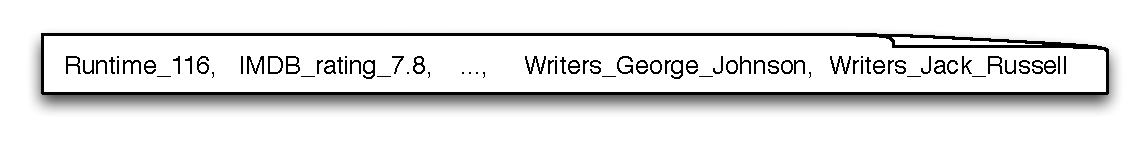
\includegraphics[width=3.2in]{imgs/w2v_example.pdf}
\caption{Sample document for $\Word2Vec$ for the Ocean's Eleven movie}
\label{fig:ocean11}
\end{center}
\end{figure}


\paragraph{Feat2Vec}
Feature representation in $\Feat2Vec$ may require a feature extraction function for each feature group.
Here, we explain how we build these functions:
\begin{itemize}
\item  \textbf{Bag of categories,  categorical, and boolean:}
For all of the categorical variables, we learn a unique $r$-dimensional embedding for each entity using a linear fully-connected layer (Equation~\ref{eq:fully_connected}).
We do not require one-hot encodings, and thus we allow multiple categories to be active; resulting in a single embedding for the group  that is the sum of  the embeddings of the subfeatures.
This is ordering-invariant:  the embedding of ``Brad Pitt'' would be the same when he appears in a movie as a principal cast member, regardless whether he was 1st  or 2nd star.
Though,  if he were listed as a director it may result in a different embedding.
\item \textbf{Text:}
We  preprocess the text by removing non alpha-numeric characters,  stopwords, and stemming the remaining words.
We then follow the same approach that we did for categorical  variables.
It would be easy to use more sophisticated methods (e.g,  convolutions).
\item \textbf{Real-valued:}
For all real-valued features, we pass these features through a 3-layer feed-forward fully connected neural network that outputs a vector of dimension $r$, which we treat as the feature's embedding.
Each intermediate layer has $r$ units with \texttt{relu} activation functions.
These real-valued features highlight one of the advantages of the $\Feat2Vec$ algorithm: using a numeric value as an input, $\Feat2Vec$ can learn a highly nonlinear relation mapping a real number to our high-dimensional embedding space. In contrast, $\Word2Vec$ would be unable to know that an IMDB rating of 5.5 is similar to  5.6.%; it would tokenize both values and treat them as independent words in a document.
\end{itemize}



\subsection{Experimental Setup}
\paragraph{Held-out set}
For our evaluation, we define a testing set that was not used to tune the parameters of the model.
For the IMDB dataset,  we  select randomly a 10\% sample of the observations that contain a director that appears at least twice in the database
\footnote{Over 90\% of the movies in the database have exactly one director, but in cases where there are multiple directors to a film, we use the first director listed in the IMDB dataset.}.
We do this to guarantee that the set of directors in the left-out dataset appear during training at least once, so that each respective algorithm can learn something about the characteristics of these directors.
For the educational dataset, our testing set only has observations for textbooks and users that appear at least 10 times in training.


\paragraph{Hyper-parameters}
For both $\Feat2Vec$ and $\Word2Vec$, we perform cross-validation on the loss function,
 by splitting the 10\% of the training data randomly into a validation set,
 to determine the number of epochs to train, and then train the full training dataset with this number of epochs.
 \footnote{because we train $\Word2Vec$ with the \texttt{gensim} python library, it is impossible to recover the output weight matrix, and so the loss function is inaccessible for an outside document set. So, we created our own loss function that measures average within-document cosine similarity of all possible token pairs. The result was that both algorithms are trained for a similar number of epochs. }
While regularization of the embeddings during training is possible, this did not dramatically change results, so we ignore this dimension of hyperparameters.

%The $\Feat2Vec$ algorithm takes approximately 5 minutes per epoch on a home desktop computer.
%The $\Feat2Vec$ model is built on the python library Keras
%Cite keras???
 For training $\Feat2Vec$  we set $\alpha_1=\alpha_2 = 3/4$ in the IMDB dataset;
 and $\alpha_1 = 0.25$ and $\alpha_2 = 0.5$  for the educational.
In each setting, $\alpha_2$ is set to the same flattening hyperparameter we use for $\Word2Vec$ to negatively sample words in a document. We learn $r=50$ dimensional embeddings under both algorithms.


\subsubsection{Results}

After training, we use the cast members associated with the movies of the test set and  attempt to predict the actual director the film was directed.
We take the sum of the cast member embeddings, and rank the directors by cosine similarity of their embeddings to the summed cast member vector.
If there is a cast member in the test dataset who did not appear in the training data, we exclude them from the summation.
For the educational dataset, we simply use the user embedding directly to get the closest textbook.

Table \ref{tab:eval} presents the results from our evaluation.
$\Feat2Vec$ sizably outperforms $\Word2Vec$  in the MPR metric.
Figure \ref{fig:cdf} shows the full distribution of rankings of the IMDB dataset, rather than summary statistics, in the form of a Cumulative Distribution Function (CDF) of all rankings calculated in the test dataset.
The graphic makes it apparent for the vast majority of the ranking space, the rank CDF of $\Feat2Vec$ is to the left of $\Word2Vec$, indicating a greater probability of a lower ranking under $\Feat2Vec$.
This is not, however, the case at the upper tail of ranking space, where it appears $\Word2Vec$ is superior.
%One might argue that while, overall, $\Feat2Vec$ appears to perform better, it is exactly that upper tail that actually matters most in practice, and so it would seem $\Word2Vec$ is more useful.
%We would argue that actually,
However, when we zoom-in on the absolute upper region of rankings (1 to 25), which might be a sensible length of ranks one might give an actual recommendation, it is the case that up until rank 8 or so, $\Feat2Vec$ outperforms $\Word2Vec$ still.
Intermediate rankings are still strong signals that our $\Feat2Vec$ algorithm is doing a better job of extracting information into embeddings, particularly those entities that appear sparsely in the training data and so are especially difficult.
In fact,  $\Feat2Vec$ predicts the actual director 2.43\% of the times, while $\Word2Vec$ only does so 1.26\% of the time, making our approach almost 2 times better in terms of Top-1 Precision metric.

\begin{table}[htb]
\footnotesize
\centering
\caption{Mean percentile rank}
\begin{tabular}{lcc}
\hline
Dataset & $\Feat2Vec$ & $\Word2Vec$ \\ \hline
IMDB & 19.36\% & 24.15\% \\
Educational & 25.2\% & 29.2\% \\
\hline
\end{tabular}
\label{tab:eval}
\end{table}

\begin{figure}[htb]
\begin{center}
\makebox[0pt]{
\begin{tikzpicture}
\node (img1) at (0,0) {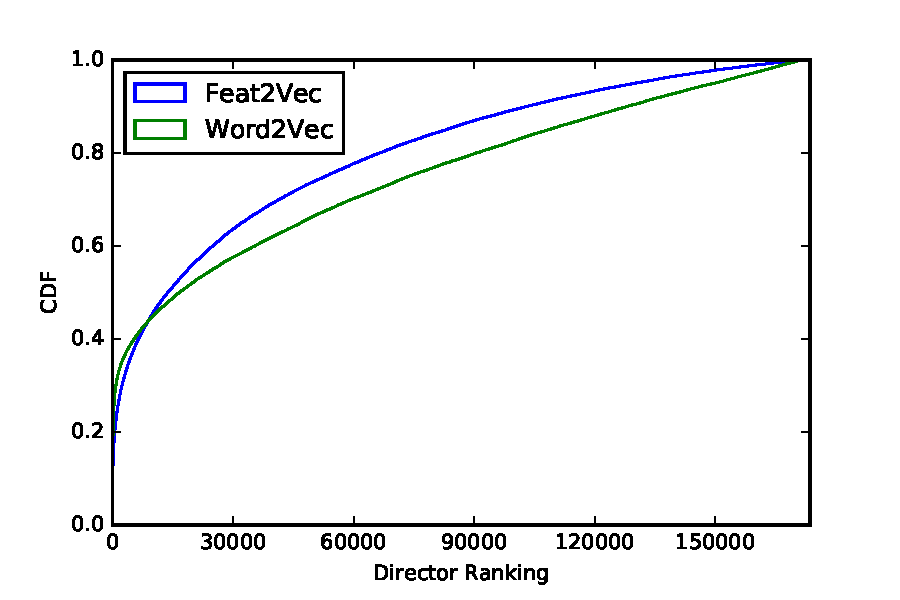
\includegraphics[scale=0.5]{rankcdf.pdf}};
\node (img2) at (1.5,-0.75) {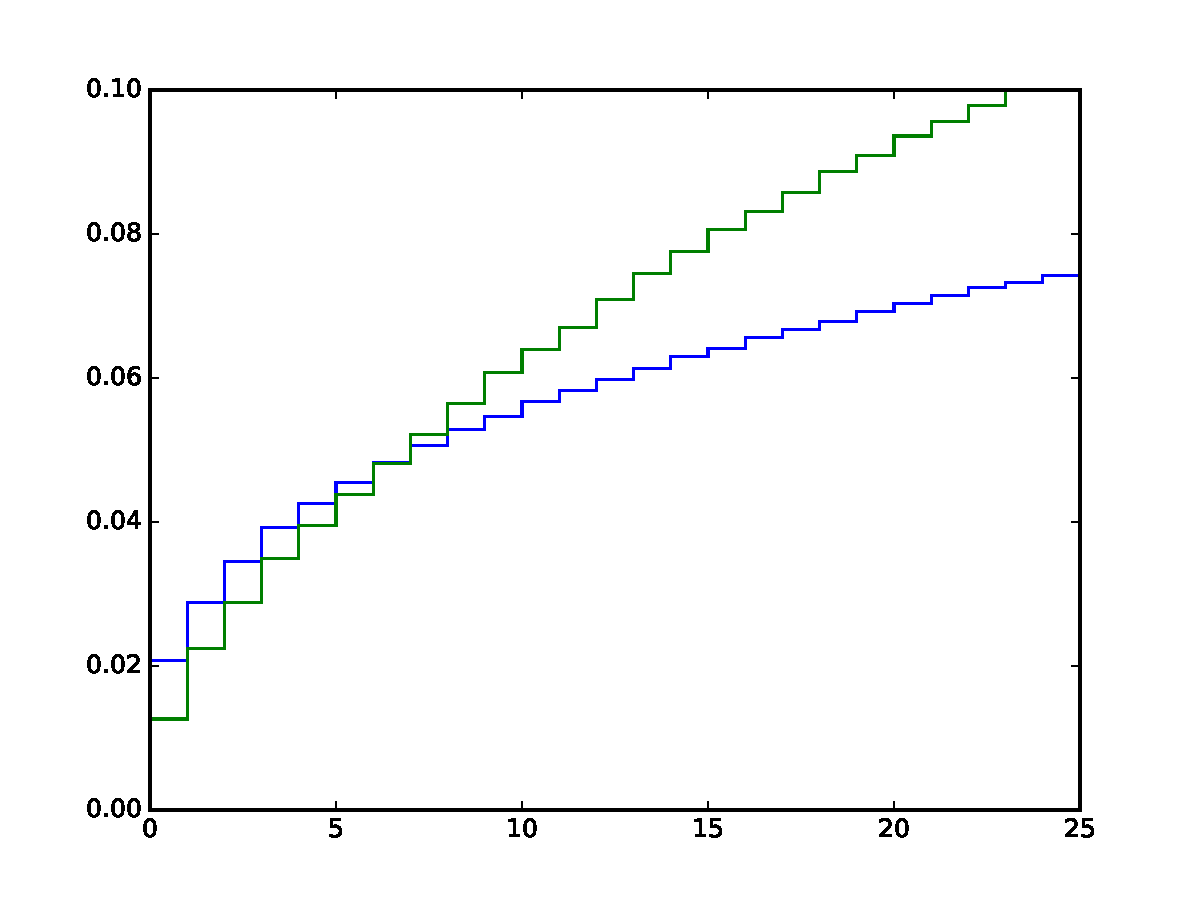
\includegraphics[scale=.25]{rankcdf_top25.pdf}};
\end{tikzpicture}
}
\end{center}
\caption{Cumulative Distribution Function of Director Rankings \\ (With Zoom-in to Top 25 Ranks)}
\label{fig:cdf}
\end{figure}

\subsection{$\Feat2Vec$ Performance with Continuous Inputs}
%^We can probably wordsmith this
%One of our goals in this work is a general-purpose algorithm that can handle arbitrary features.
%We study  $\Feat2Vec$'s performance on a continuous feature. %non-categorical features, we evaluate the embeddings calculated using
We now focus on how well $\Feat2Vec$ performs on a real-valued feature with a complex feature extraction function.
We evaluate the prediction of the real-valued rating of movies in the test dataset by choosing the IMDB rating embedding most similar\footnote{As before, the metric is cosine similarity.} to the embedding of the movie's director, and compute the Root Mean Squared Error (RMSE) of the predicted rating in the test dataset. We also vary $\alpha_1$, the flattening hyperparameter for feature sampling, to see what the effect this hyperparameter has on our performance. Intuitively, a low $\alpha_1$ will greatly improve the quality of the ratings embeddings learned, since it has relatively few parameters and is otherwise sampled infrequently. At the same time, with low $\alpha_1$ the director feature will be sampled less since it is one of the most complex features to learn, so the learned director embeddings may be of poorer quality. Figure \ref{fig:ratings} displays the results of our experiment, benchmarked against $\Word2Vec$'s performance in the prediction task. We also show as a baseline the RMSE of a random uniform variable over the range of possible ratings (0 to 10). As is evident from the plot, $\Word2Vec$ performs a bit better than a random prediction, but is also handily outperformed by $\Feat2Vec$ across all hyper-parameter settings.
%There is no clear relation between $\alpha_1$ and the RMSE, suggesting
The algorithm's performance does not seem very sensitive to the hyperparameter choice.



\begin{figure}
\centering
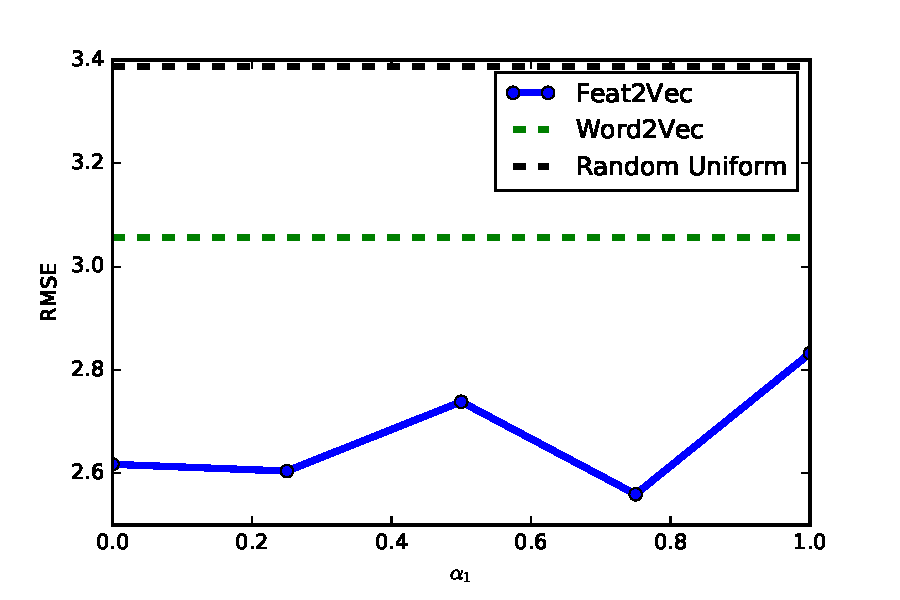
\includegraphics[scale=.5]{../paper/output/ratingsRankingRMSE.pdf}
\caption{RMSE in Ratings Task as a Function of $\alpha_1$}
\label{fig:ratings}
\end{figure}

\section{Relation to Prior Work}
Algorithms that calculate continuous representations of entities other than words have been studied in the context of  bioinformatics for biological sequences~\cite{biovec},
or in machine translation for embeddings of complete sentences~\cite{kiros2015skip}.
We recently discovered a promising direction for an algorithm still in development called StarSpace~\cite{wu2017starspace} with similar goals from ours.
Even though they intend to be able to embed all types of features, at the time of the writing of this paper, their pre-print method was limited to only work for bag of words.
While $\Feat2Vec$ can jointly learn embeddings for all feature values in a dataset,  StarSpace samples a single arbitrary feature.
Our preliminary experiments suggest that sampling a single feature does not produce embeddings that generalize well.
Nonetheless, a limitation of our work is that we do not compare with StarSpace, which future work may decide to do.

\section{Conclusion}
%Embeddings are useful tools in in Artificial Intelligence.
Motivated by the success of $\Word2Vec$, this paper proposes a novel algorithm that relies on Structured Deep Factorization Machines with implicit sampling to learn general purpose embedding representations of different types of features.
Future work could study how to reduce the amount of  human knowledge our approach requires;
for example by automatically grouping features into entities, or by automatically choosing a feature extraction function.
These ideas can extend to our codebase that we make available
\footnote{The code for the $\Feat2Vec$ algorithm is available \href{https://www.dropbox.com/sh/wdr2sgt0z9gj6kb/AABlzw7QhteTYViSoMk3CDZpa?dl=0}{here} and the empirical experiments for the IMDB data can be found
\href{https://www.dropbox.com/sh/uc07ng403i4ss9a/AAAPshFzdOug_ooeLn4SGR3Ua?dl=0}{here}
}.

Our evaluation is limited to two datasets---a public dataset that is freely available,  and a proprietary one that we are unable to distribute.
Though further experimentation is definitely necessary, we believe that our results are extremely encouraging.
$\Feat2Vec$'s embeddings are able to capture relationships across features that can be twice as better as $\Word2Vec$ on some evaluation metrics.

$\Feat2Vec$ exploits the structure of a datasets to learn embeddings in a way that is structurally more sensible than existing methods.
The sampling method, and loss function that we use have interesting theoretical properties.
To the extent of our knowledge, $\Feat2Vec$  is the first method able to calculate continuous representations of data with arbitrary feature types.




%\pagebreak


{
%\footnotesize
%\setlength{\bibsep}{0pt plus 0.25ex}
\bibliography{joseg}
\bibliographystyle{iclr2018_conference}
}

\pagebreak
\appendix
\renewcommand\thefigure{A.\arabic{figure}}
\setcounter{figure}{0}
\section{Appendixes}
\begin{figure}[h]
\centering
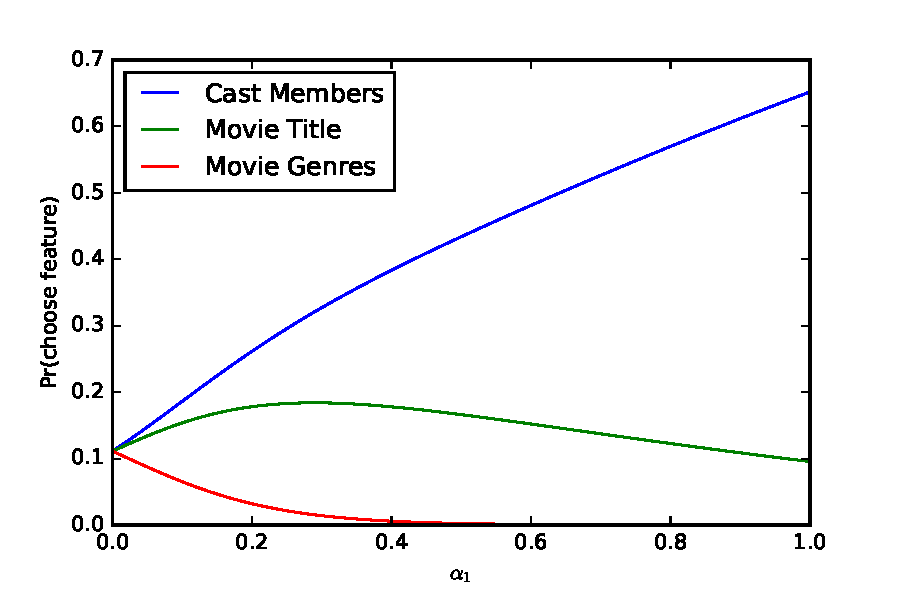
\includegraphics[scale=.6]{../paper/output/samplingprobs.pdf}
\caption{Feature Sampling Probabilities as a Function of $\alpha_1$}
\label{fig:alpha}
\end{figure}

\subsection{Proof to Theorem \ref{thm:proof}}
\begin{theorem}
The gradient for learning embeddings with $\Feat2Vec$ is a convex combination of the gradient from $p$ targeted Factorization Machines for each feature in the data.
\label{thm:proof}
\end{theorem}
\begin{proof}
Let $S^+_{\upkappa_i}$ denote the positively labeled records whose corresponding negative samples resample feature $\upkappa_i$. We can express the loss function $L(.)$, the binary cross-entropy of the data given the $\Feat2Vec$ model, as follows:

\begin{align*}
 L(S^+ | \vec{\phi} )  =&   \frac{1}{|S^+|} \sum_{\vect{x}^+ \in S^+} \Big(\log(\tilde p(Y=1|\vec{\phi},\vect{x}^+  ) ) + \sum_{\vect{x}^{\,-}\sim \q(.|\vect{x}^+)}^k \log(\tilde p(Y=0|\vec{\phi},\vect{x}^{\,-})) \Big) \\
  =&  \frac{1}{|S^+|} \sum_{\vect{x}^+ \in S^+} \Big( \log(\tilde p(Y=1|\vec{\phi},\vect{x}^+, \vect{x}^+ \in S^+_{\upkappa_i} )p(\vect{x}^+ \in S^+_{\upkappa_i}) ) \\ &
   + \sum_{\vect{x}^{\,-} \sim \q(.|\vect{x}^+)}^k \log(\tilde p(Y=0|\vec{\phi},\vect{x}^{\,-},\vect{x}^+ \in S^+_{\upkappa_i})p(\vect{x}^+ \in S^+_{\upkappa_i})) \Big) \\
  =&  \frac{1}{|S^+|}\sum_{i=1}^p \sum_{\vect{x}^+ \in S^+_{\upkappa_i}} \Big( \log(\frac{e^{s(\vect{x}^+,\vec{\phi}) } p(\vect{x}^+ \in S^+_{\upkappa_i})}{e^{s(\vect{x}^+,\vec{\phi}) } + P_{\q}(\vect{x}^+ |\vect{x}^+, \vect{x}^+ \in S^+_{\upkappa_i}) }) \\ &
  +  \sum_{\vect{x}^{\,-} \sim \q(.|\vect{x}^+,\vect{x}^+ \in S^+_{\upkappa_i})}^k \log(\frac{ P_{\q}(\vect{x}^{\,-} |\vect{x}^+, \vect{x}^+ \in S^+_{\upkappa_i})p(\vect{x}^+ \in S^+_{\upkappa_i})}{e^{s(\vect{x}^{\,-},\vec{\phi}) } + P_{\q}(\vect{x}^{\,-}|\vect{x}^+, \vect{x}^+ \in S^+_{\upkappa_i})}) \Big) \\
  \intertext{Note now that $P_{\q}(\vect{x}|\vect{x}^+,\vect{x}^+ \in S^+_{\upkappa_i})$ is simply the probability of the record's feature value $\vect{x}_{f}$ under the second step noise distribution $\q_2(\mathrm{X_{f}},\alpha_2)$:
   $P_{\q}(\vect{x}|\vect{x}^+,\vect{x}^+ \in S^+_{\upkappa_i}) = P_{\q_2}(\vect{x}_{f})$}\\
=&  \frac{1}{|S^+|}\sum_{i=1}^p \sum_{\vect{x}^+ \in S^+_{\upkappa_i}} \Big( \log(\frac{e^{s(\vect{x}^+,\vec{\phi}) } p(\vect{x}^+ \in S^+_{\upkappa_i})}{e^{s(\vect{x}^+,\vec{\phi}) } + P_{\q_2}(\vect{x}^+_{\upkappa_i}) } ) + \sum_{\vect{x}^{\,-} \sim \q(.|\vect{x}^+,i\in S^+_{\upkappa_i})}^k \log(\frac{  P_{\q_2}(\vect{x}^{\,-}_{f})p(\vect{x}^+ \in S^+_{\upkappa_i})}{e^{s(\vect{x}^{\,-},\vec{\phi}) } + P_{\q_2}(\vect{x}^{\,-}_{f})) } \Big) \\
   = & \frac{1}{|S^+|}\sum_{i=1}^p \sum_{\vect{x}^+ \in S^+_{\upkappa_i}} \Big( \log(\frac{e^{s(\vect{x}^+,\vec{\phi}) }}{e^{s(\vect{x}^+,\vec{\phi}) } + P_{\q_2}(\vect{x}^+_{\upkappa_i}) }) + \log(p(\vect{x}^+ \in S^+_{\upkappa_i})^{k+1})\\
  &   +  \sum_{\vect{x}^{\,-} \sim \q(.|\vect{x}^+,\vect{x}^+ \in S^+_{\upkappa_i})}^k \log(\frac{ P_{\q_2}(\vect{x}^{\,-}_{f})}{e^{s(\vect{x}^{\,-},\vec{\phi}) } + P_{\q_2}(\vect{x}^{\,-}_{f})})   \Big) \\
\intertext{We now drop the term containing the probability of assignment to a feature type $p(\vect{x}^+ \in S^+_{\upkappa_i})$ since it is outside of the learned model parameters $\vec{\phi}$ and fixed in advance:}\\
    \propto & \frac{1}{|S^+|} \sum_{i=1}^p \sum_{\vect{x}^+ \in S^+_{\upkappa_i}} \Big( \log(\frac{e^{s(\vect{x}^+,\vec{\phi}) }}{e^{s(\vect{x}^+,\vec{\phi}) } + P_{\q_2}(\vect{x}^+_{\upkappa_i}) }) + \sum_{\vect{x}^{\,-} \sim \q(.|\vect{x}^+,\vect{x}^+ \in S^+_{\upkappa_i})}^k \log(\frac{ P_{\q_2}(\vect{x}^{\,-}_{f})}{e^{s(\vect{x}^{\,-},\vec{\phi}) } + P_{\q_2}(\vect{x}^{\,-}_{f})}) \Big) \\
    \xrightarrow[|S^+|\rightarrow \infty]{ }  & \sum_{i=1}^p p(\vect{x}^+ \in S^+_{\upkappa_i}) E\Big[ \log(\frac{e^{s(\vect{x}^+,\vec{\phi}) }}{e^{s(\vect{x}^+,\vec{\phi}) } + P_{\q_2}(\vect{x}^+_{\upkappa_i}) }) + \sum_{\vect{x}^{\,-} \sim \q(.|\vect{x}^+,\vect{x}^+ \in S^+_{\upkappa_i})}^k \log(\frac{ P_{\q_2}(\vect{x}^{\,-}_{f})}{e^{s(\vect{x}^{\,-},\vec{\phi}) } + P_{\q_2}(\vect{x}^{\,-}_{f})}) \Big] \\
   & = \sum_{i=1}^p p(\vect{x}^+ \in S^+_{\upkappa_i}) E\Big[ L(\vec{x} |\vec{\phi}, \text{target = $f$}) \Big]
\end{align*}

Thus, the loss function is just a convex combination  of the loss functions of the targeted classifiers for each of the $p$ features, and by extension so is the gradient since:

\[\frac{\partial }{\partial \phi}\sum_{i=1}^p p(\vect{x}^+ \in S^+_{\upkappa_i}) E\Big[ L(\vec{x} |\vec{\phi}, \text{target = $f$}) \Big] =
 \sum_{i=1}^p p(\vect{x}^+ \in S^+_{\upkappa_i}) \frac{\partial }{\partial \phi}E\Big[ L(\vec{x} |\vec{\phi}, \text{target = $f$}) \Big]\]
 Thus the algorithm will, at each step, learn a convex combination of the gradient for a targeted classifier on feature $f$, with weights proportional to the feature type sampling probabilities in step 1 of the sampling algorithm.
\end{proof}

\end{document}
